%% abtex2-modelo-trabalho-academico.tex, v-1.9.2 laurocesar
%% Copyright 2012-2014 by abnTeX2 group at http://abntex2.googlecode.com/ 
%%
%% This work may be distributed and/or modified under the
%% conditions of the LaTeX Project Public License, either version 1.3
%% of this license or (at your option) any later version.
%% The latest version of this license is in
%%   http://www.latex-project.org/lppl.txt
%% and version 1.3 or later is part of all distributions of LaTeX
%% version 2005/12/01 or later.
%%
%% This work has the LPPL maintenance status `maintained'.
%% 
%% The Current Maintainer of this work is the abnTeX2 team, led
%% by Lauro César Araujo. Further information are available on 
%% http://abntex2.googlecode.com/
%%
%% This work consists of the files abntex2-modelo-trabalho-academico.tex,
%% abntex2-modelo-include-comandos and abntex2-modelo-references.bib
%%


% ------------------------------------------------------------------------
% ------------------------------------------------------------------------
% abnTeX2: Modelo de Trabalho Academico (tese de doutorado, dissertacao de
% mestrado e trabalhos monograficos em geral) em conformidade com 
% ABNT NBR 14724:2011: Informacao e documentacao - Trabalhos academicos -
% Apresentacao
% ------------------------------------------------------------------------
% ------------------------------------------------------------------------

\documentclass[
	% -- opções da classe memoir --
	12pt,				% tamanho da fonte
	openany,			% capítulos começam em pág ímpar (insere página vazia caso preciso)
	oneside,			% para impressão em verso e anverso. Oposto a oneside
	a4paper,			% tamanho do papel. 
	% -- opções da classe abntex2 --
	chapter=TITLE,		% títulos de capítulos convertidos em letras maiúsculas
	section=TITLE,		% títulos de seções convertidos em letras maiúsculas
	subsection=TITLE,	% títulos de subseções convertidos em letras maiúsculas
	subsubsection=TITLE,% títulos de subsubseções convertidos em letras maiúsculas
	% -- opções do pacote babel --
	english,			% idioma adicional para hifenização
	brazil				% o último idioma é o principal do documento
	]{iesb-abntex2}
% ---
% Pacotes básicos 
% ---
\usepackage{lmodern}			% Usa a fonte Latin Modern			
\usepackage[T1]{fontenc}		% Selecao de codigos de fonte.
\usepackage[utf8]{inputenc}		% Codificacao do documento (conversão automática dos acentos)
\usepackage{lastpage}			% Usado pela Ficha catalográfica
\usepackage{indentfirst}		% Indenta o primeiro parágrafo de cada seção.
\usepackage{color}				% Controle das cores
\usepackage{graphicx}			% Inclusão de gráficos
\usepackage{microtype} 			% para melhorias de justificação
% ---
		
% ---
% Pacotes adicionais, usados apenas no âmbito do Modelo Canônico do abnteX2
% ---
\usepackage{lipsum}				% para geração de dummy text
% ---

% ---
% Pacotes de citações
% ---

\usepackage[brazilian,hyperpageref]{backref}	 % Paginas com as citações na bibl
%\usepackage[alf]{abntex2cite}	% Citações padrão ABNT
\usepackage[alf,abnt-and-type=e]{abntex2cite}

% --- 
% CONFIGURAÇÕES DE PACOTES
% --- 

% ---
% Configurações do pacote backref
% Usado sem a opção hyperpageref de backref
\renewcommand{\backrefpagesname}{Citado na(s) página(s):~}
% Texto padrão antes do número das páginas
\renewcommand{\backref}{}
% Define os textos da citação
\renewcommand*{\backrefalt}[4]{
	\ifcase #1 %
		Nenhuma citação no texto.%
	\or
		Citado na página #2.%
	\else
		Citado #1 vezes nas páginas #2.%
	\fi}%
% ---

% ---
% Informações de dados para CAPA e FOLHA DE ROSTO
% ---
\titulo{Aprendizado de Máquina aplicado\\ à Genômica Funcional}
\autor{Ênio José Ferreira Júnior e Jonas Siqueira Ramos}
\local{Brasília -- DF}
\data{2019}
\orientador{Letícia Maia Toledo Zoby}
% \coorientador{Equipe \abnTeX}
%\instituicao{%
%  Universidade do Brasil -- UBr
%  \par
%  Faculdade de Arquitetura da Informação
%  \par
%  Programa de Pós-Graduação}
\tipotrabalho{Monografia (Graduação)}
% O preambulo deve conter o tipo do trabalho, o objetivo, 
% o nome da instituição e a área de concentração 
\preambulo{Trabalho de Conclusão de Curso apresentado ao Instituto de Educação Superior de Brasília, DF, como parte dos requisitos para obtenção do título de Bacharel em Ciência da Computação.}
% ---


% ---
% Configurações de aparência do PDF final

% alterando o aspecto da cor azul
\definecolor{blue}{RGB}{41,5,195}
\definecolor{black}{RGB}{0, 0, 0}

% informações do PDF
\makeatletter
\hypersetup{
     	%pagebackref=true,
		pdftitle={\@title}, 
		pdfauthor={\@author},
    	pdfsubject={\imprimirpreambulo},
	    pdfcreator={LaTeX with abnTeX2},
		pdfkeywords={abnt}{latex}{abntex}{abntex2}{trabalho acadêmico}, 
		colorlinks=false,       		% false: boxed links; true: colored links
    	linkcolor=black,          	% color of internal links
    	citecolor=black,        		% color of links to bibliography
    	filecolor=black,      		% color of file links
		urlcolor=black,
		bookmarksdepth=4
}
\makeatother
% --- 

% ---
% compila o indice
% ---
\makeindex
% ---

% ----
% Início do documento
% ----
\begin{document}

% Retira espaço extra obsoleto entre as frases.
\frenchspacing 

% ----------------------------------------------------------
% ELEMENTOS PRÉ-TEXTUAIS
% ----------------------------------------------------------
\pretextual

% ---
% Capa
% ---
\imprimircapa
% ---

% ---
% Folha de rosto
% (o * indica que haverá a ficha bibliográfica)
% ---
\imprimirfolhaderosto*
% ---

% ---
% Inserir a ficha bibliografica
% ---

% Isto é um exemplo de Ficha Catalográfica, ou ``Dados internacionais de
% catalogação-na-publicação''. Você pode utilizar este modelo como referência. 
% Porém, provavelmente a biblioteca da sua universidade lhe fornecerá um PDF
% com a ficha catalográfica definitiva após a defesa do trabalho. Quando estiver
% com o documento, salve-o como PDF no diretório do seu projeto e substitua todo
% o conteúdo de implementação deste arquivo pelo comando abaixo:
%
% \begin{fichacatalografica}
%     \includepdf{fig_ficha_catalografica.pdf}
% \end{fichacatalografica}
%\begin{fichacatalografica}
%	\vspace*{\fill}					% Posição vertical
%	\hrule							% Linha horizontal
%	\begin{center}					% Minipage Centralizado
%	\begin{minipage}[c]{12.5cm}		% Largura
	
%	\imprimirautor
	
%	\hspace{0.5cm} \imprimirtitulo  / \imprimirautor. --
%	\imprimirlocal, \imprimirdata-
	
%	\hspace{0.5cm} \pageref{LastPage} p. : il. (algumas color.) ; 30 cm.\\
	
%	\hspace{0.5cm} \imprimirorientadorRotulo~\imprimirorientador\\
	
%	\hspace{0.5cm}
%	\parbox[t]{\textwidth}{\imprimirtipotrabalho~--~\imprimirinstituicao,
%	\imprimirdata.}\\
	
%	\hspace{0.5cm}
%		1. Palavra-chave1.
%		2. Palavra-chave2.
%		I. Orientadora.
%		II. Universidade xxx.
%		III. Faculdade de xxx.
%		IV. Título\\ 			
	
%	\hspace{8.75cm} CDU 02:141:005.7\\
	
%	\end{minipage}
%	\end{center}
%	\hrule
%\end{fichacatalografica}
% ---

% ---
% Inserir folha de aprovação
% ---

% Isto é um exemplo de Folha de aprovação, elemento obrigatório da NBR
% 14724/2011 (seção 4.2.1.3). Você pode utilizar este modelo até a aprovação
% do trabalho. Após isso, substitua todo o conteúdo deste arquivo por uma
% imagem da página assinada pela banca com o comando abaixo:
%
% \includepdf{folhadeaprovacao_final.pdf}
%
\begin{folhadeaprovacao}

  \begin{center}
    {\IESBheader\vspace*{1cm}}
    %{\ABNTEXchapterfont\large\imprimircurso}
    {\ABNTEXchapterfont\large\imprimirautor}

    \vspace*{\fill}\vspace*{\fill}
    \begin{center}
      \ABNTEXchapterfont\bfseries\Large{Aprendizado de Máquina aplicado \par à Genômica Funcional}
    \end{center}
    \vspace*{\fill}
    
    \hspace{.45\textwidth}
    \begin{minipage}{.5\textwidth}
        \imprimirpreambulo
    \end{minipage}
    \vspace*{\fill}
    
    \ABNTEXchapterfont\Large{Brasília, \imprimirdataapresentacao.}
    
    \vspace*{\fill}
   \end{center}
   
    \begin{center}
      \ABNTEXchapterfont\Large{Banca examinadora:}
    \end{center}
   
        
   %Trabalho aprovado. \imprimirlocal, 24 de novembro de 2019:

   \assinatura{\textbf{Prof. Dra.} - Orientadora} 
   \assinatura{\textbf{Prof.} - Membro}
   \assinatura{\textbf{Prof.} - Membro}
   %\assinatura{\textbf{Professor} \\ Convidado 3}
   %\assinatura{\textbf{Professor} \\ Convidado 4}
      
   %\begin{center}
   % \vspace*{0.5cm}
   % {\large\imprimirlocal}
   % \par
   % {\large\imprimirdata}
   % \vspace*{1cm}
   %\end{center}
  
\end{folhadeaprovacao}
% ---

% ---
% Dedicatória
% ---
%\begin{dedicatoria}
%   \vspace*{\fill}
%   \centering
%   \noindent
%   \textit{ Este trabalho é dedicado às crianças adultas que,\\
%   quando pequenas, sonharam em se tornar cientistas.} \vspace*{\fill}
%\end{dedicatoria}
% ---

% ---
% Agradecimentos
% ---
%\begin{agradecimentos}
%Os agradecimentos principais são direcionados à Gerald Weber, Miguel Frasson,
%Leslie H. Watter, Bruno Parente Lima, Flávio de Vasconcellos Corrêa, Otavio Real
%Salvador, Renato Machnievscz\footnote{Os nomes dos integrantes do primeiro
%projeto abn\TeX\ foram extraídos de
%\url{http://codigolivre.org.br/projects/abntex/}} e todos aqueles que
%contribuíram para que a produção de trabalhos acadêmicos conforme
%as normas ABNT com \LaTeX\ fosse possível.

%Agradecimentos especiais são direcionados ao Centro de Pesquisa em Arquitetura
%da Informação\footnote{\url{http://www.cpai.unb.br/}} da Universidade de
%Brasília (CPAI), ao grupo de usuários
%\emph{latex-br}\footnote{\url{http://groups.google.com/group/latex-br}} e aos
%novos voluntários do grupo
%\emph{\abnTeX}\footnote{\url{http://groups.google.com/group/abntex2} e
%\url{http://abntex2.googlecode.com/}}~que contribuíram e que ainda
%contribuirão para a evolução do \abnTeX.

%\end{agradecimentos}
% ---

% ---
% Epígrafe
% ---
%\begin{epigrafe}
%    \vspace*{\fill}
%	\begin{flushright}
%		\textit{``Não vos amoldeis às estruturas deste mundo, \\
%		mas transformai-vos pela renovação da mente, \\
%		a fim de distinguir qual é a vontade de Deus: \\
%		o que é bom, o que Lhe é agradável, o que é perfeito.\\
%		(Bíblia Sagrada, Romanos 12, 2)}
%	\end{flushright}
%\end{epigrafe}
% ---

% ---
% RESUMOS
% ---

% resumo em português
\setlength{\absparsep}{18pt} % ajusta o espaçamento dos parágrafos do resumo
\begin{resumo}
 Segundo a \citeonline[3.1-3.2]{NBR6028:2003}, o resumo deve ressaltar o
 objetivo, o método, os resultados e as conclusões do documento. A ordem e a extensão
 destes itens dependem do tipo de resumo (informativo ou indicativo) e do
 tratamento que cada item recebe no documento original. O resumo deve ser
 precedido da referência do documento, com exceção do resumo inserido no
 próprio documento. (\ldots) As palavras-chave devem figurar logo abaixo do
 resumo, antecedidas da expressão Palavras-chave:, separadas entre si por
 ponto e finalizadas também por ponto.

 \textbf{Palavras-chaves}: latex. abntex. editoração de texto.
\end{resumo}

% resumo em inglês
\begin{resumo}[Abstract]
 \begin{otherlanguage*}{english}
   This is the english abstract.

   \vspace{\onelineskip}
 
   \noindent 
   \textbf{Key-words}: latex. abntex. text editoration.
 \end{otherlanguage*}
\end{resumo}

% ---

% ---
% inserir lista de ilustrações
% ---
\pdfbookmark[0]{\listfigurename}{lof}
\listoffigures*
\cleardoublepage
% ---

% ---
% inserir lista de tabelas
% ---
%\pdfbookmark[0]{\listtablename}{lot}
%\listoftables*
%\cleardoublepage
% ---

% ---
% inserir lista de abreviaturas e siglas
% ---
\begin{siglas}
  \item[ARN] Ácido Ribonucleico
  \item[RNA] Redes Neurais Artificiais
  \item[SBC] Sistemas Baseados em Conhecimento
  \item[SE] Sistemas Especialistas
\end{siglas}
% ---

% ---
% inserir lista de símbolos
% ---
%\begin{simbolos}
%  \item[$ \Gamma $] Letra grega Gama
%  \item[$ \Lambda $] Lambda
%  \item[$ \zeta $] Letra grega minúscula zeta
%  \item[$ \in $] Pertence
%\end{simbolos}
% ---

% ---
% inserir o sumario
% ---
\pdfbookmark[0]{\contentsname}{toc}
\tableofcontents*
\cleardoublepage
% ---

% ----------------------------------------------------------
% ELEMENTOS TEXTUAIS
% ----------------------------------------------------------
\textual

et% ----------------------------------------------------------
% Introdução 
% ----------------------------------------------------------
\chapter[Introdução]{Introdução}
%\addcontentsline{toc}{chapter}{Introdução}
% ----------------------------------------------------------

Este documento e seu código-fonte são exemplos de referência de uso da classe
\textsf{abntex2} e do pacote \textsf{abntex2cite}. O documento 
exemplifica a elaboração de trabalho acadêmico (tese, dissertação e outros do
gênero) produzido conforme a ABNT NBR 14724:2011 \emph{Informação e documentação
- Trabalhos acadêmicos - Apresentação}.

A expressão ``Modelo Canônico'' é utilizada para indicar que \abnTeX\ não é
modelo específico de nenhuma universidade ou instituição, mas que implementa tão
somente os requisitos das normas da ABNT. Uma lista completa das normas
observadas pelo \abnTeX\ é apresentada em \citeonline{abntex2classe}.

Sinta-se convidado a participar do projeto \abnTeX! Acesse o site do projeto em
\url{http://abntex2.googlecode.com/}. Também fique livre para conhecer,
estudar, alterar e redistribuir o trabalho do \abnTeX, desde que os arquivos
modificados tenham seus nomes alterados e que os créditos sejam dados aos
autores originais, nos termos da ``The \LaTeX\ Project Public
License''\footnote{\url{http://www.latex-project.org/lppl.txt}}.

Encorajamos que sejam realizadas customizações específicas deste exemplo para
universidades e outras instituições --- como capas, folha de aprovação, etc.
Porém, recomendamos que ao invés de se alterar diretamente os arquivos do
\abnTeX, distribua-se arquivos com as respectivas customizações.
Isso permite que futuras versões do \abnTeX~não se tornem automaticamente
incompatíveis com as customizações promovidas. Consulte
\citeonline{abntex2-wiki-como-customizar} par mais informações.

Este documento deve ser utilizado como complemento dos manuais do \abnTeX\ 
\cite{abntex2classe,abntex2cite,abntex2cite-alf} e da classe \textsf{memoir}
\cite{memoir}. 

Esperamos, sinceramente, que o \abnTeX\ aprimore a qualidade do trabalho que
você produzirá, de modo que o principal esforço seja concentrado no principal:
na contribuição científica.

Equipe \abnTeX 

Lauro César Araujo

\section{Justificativa}

\section{Problema}

\section{Objetivos}

\section{Conteúdo e Organização}

\chapter{Revisão Bibliográfica}

Esta seção tem como objetivo apresentar os conhecimentos necessários para o claro entendimento deste trabalho.

\section{Aprendizado de Máquina}
Na década de 1970, a disseminação de técnicas no ramo da inteligência artificial (IA), tiveram um avanço na solução de problemas reais. A fim de solucionar tais problemas, muitas vezes eram necessários especialistas de um dado domínio para fornecer conhecimento, para com isso, posteriormente ser estruturado computacionalmente e ser desenvolvido a solução. Tal conhecimento era estruturado por um conjunto de regras lógicas em programas de computador, que ficaram conhecidos como Sistemas Especialistas (SE) ou Sistemas Baseados em Conhecimento (SBC). Porém, quando depende-se de um ser humano, alguns fatores podem ocorrer no processo de aquisição do conhecimento, que é a subjetividade ou até mesmo a dificuldade de transmitir o conhecimento por parte do especialista, podendo assim tornar o processo ineficaz por falta de informações.

Com o passar do tempo e o avanço da tecnologia, a quantidade de dados cresceu exponencialmente, acarretando no surgimento de problemas mais complexos a serem resolvidos computacionalmente. Com isso, surge uma maior necessidade de se ter ferramentas computacionais mais independentes com a finalidade de reduzir a interferência humana e a dependência de especialistas. Tais ferramentas, devem ser capazes de gerar uma saída, baseado em experiências e dados refentes ao passado, ou hipóteses, a fim de solucionar um dado problema. Um exemplo disso é a sugestão de produtos que um cliente provavelmente possa se interessar. Essa sugestão pode ser feita através de produtos previamente comprados pelo cliente, gerando hipóteses de outros produtos através de algum padrão encontrado entre outros produtos, podendo ser alguns deles: marca, categoria ou até mesmo faixa de preço. Esse processo de indução da hipótese pela ferramente computacional, é chamado de Aprendizado de Máquina (AM).

\subsection{Aprendizado de Máquina aplicado à Biologia}
No ramo biologia tem se tornado frequente ver aplicações com o intuito de bla bla bla

\subsection{Redes Neurais Artificiais}
* Falar sobre história de rede neural? Aplicações atualmente?

* Estrutura de uma rede neural.

* Falar de ML aplicado à biologia e o que pode ser feito.

\subsection{Técnicas de validação}
* Técnicas de validação

\subsection{Métricas}
* Métricas

\subsection{Algoritmos}
* Falar dos algoritmos que iremos utilizar.

Rede Neural RNA1
RNA2
\section{Biologia Molecular}

\cite{brock2010microbiologia}

\cite{thompson2008genetica}

* 
\section{Trabalhos Correlatos}

Em \citeauthoronline{tanaka2013adaptaccao} (\citeyear{tanaka2013adaptaccao}), é utilizado uma adaptação do método \textit{Binary Relevance} com árvores de decisão para classificação multirrotular de proteínas. Por conta da base de dados ser estruturada de forma hierárquica, a classificação foi feita em cada um dos 4 níveis de classificação da base, chegando a ter mais de 95\% de acurácia em alguns rótulos.

Segundo \citeauthoronline{resende2018combinaccao} (\citeyear{resende2018combinaccao}) propõe o uso de redes complexas com algoritmos de classificação para aplicação em problemas de classificação multirrótulo, utilizando-se de conceitos em teoria dos grafos para levar a consideração a topologia dos dados e, assim, melhorar a inferência dos rótulos. Em uma das bases testadas, foi possível observar um ganho de aproximadamente 20\% em acurácia com o uso desta técnica.

Em \citeauthoronline{ururahy2018classificaccao} (\citeyear{ururahy2018classificaccao}) é empregado o uso de classificação multirrótulo para classificar os possíveis gêneros de um filme a partir do sumário. No trabalho, foram escolhidos os 500 termos mais frequentes dos resumos para a construção do classificador, usando, para isso, o método \textit{Binary Relevance} e o algoritmo \texttt{Naive Bayes}. A acurácia máxima, média e mínima dentre os rótulos utilizados foram de 76\%, 66\% e 62\%, respectivamente. 

\citeauthoronline{coelho2018prediccao} (\citeyear{coelho2018prediccao}) faz o uso de máquinas de vetor de suporte e RNAa para predizer regiões promotoras. Os testes foram efetuados com dados da bactéria \textit{Bacillus subtilis}, uma Gram-positiva, já que “grande parte dos trabalhos sobre promotores bacterianos estão restritos a bactérias Gram-negativas”, além de existir “poucos dados de Gram-positivas na literatura” \cite{coelho2018prediccao}. O estudo concluiu que os resultados observados estão de acordo com a literatura, chegando a obter 98.57\% e 97.69\% de acurácia, no caso de duas redes neurais com configurações similares, e 93.20\% e 95.63\% de acurácia, no caso de máquinas de vetor de suporte com diferentes \texttt{kernels}.

 Em \citeauthoronline{zhang2014review} (\citeyear{zhang2014review}) é feito um estudo do estado da arte em aprendizagem multirrótulo, abordando os fundamentos, um detalhamento técnico entre 8 algoritmos e faz um breve comparativo com a aprendizagem supervisionada. O autor expõe a importância e a relevância de em certos momentos, termos uma instância associada à mais de um rótulo. Os algoritmos citados e expostos pelo autor, são: \textit{Binary Relevance}, \textit{Classifier Chains}, \textit{Calibrated Label Ranking}, \textit{Random k-Labelsets}, a adaptação do \textit{k-Nearest Neighbor} (kNN) para classificação multirrótulo (ML-kNN), \textit{Multi-Label Decision Tree} (ML-DT), \textit{Ranking Support Vector Machine} (Rank-SVM) e \textit{Collective Multi-Label Classifier} (CML).

\citeauthoronline{gibaja2014} (\citeyear{gibaja2014}) fazem uma compilação sobre o estado da arte em classificação multirrótulo. A pesquisa apresenta um olhar da área sobre diversas perspectivas, tais como: aplicações, estudos em andamento, a CMR na literatura, os principais algoritmos existentes, métricas de avaliação, entre outros.

\citeauthoronline{liu2015multi} (\citeyear{liu2015multi}) apresentam um estudo comparativo entre diferentes algoritmos de classificação multirrótulo aplicado à textos de microblogs, utilizando, para isso, duas bases de dados distintas: HR e AI
\footnote{As bases de dados HR e AI são compostas de comentários sobre dois incidentes que aconteceram na China, os quais ganharam atenção nacional na época em que aconteceram. Mais informações em \loccit{liu2015multi}}. 
O processo proposto é dividido em três partes: segmentação textual, em que um determinado texto é dividido em pequenas frases ou palavras; extração de características, em que o resultado da etapa anterior é mapeado com 3 dicionários de sentimentos para descobrir os possíveis sentimentos de uma palavra, assim como a força e a polarização de tal sentimento; e, por último, a classificação multirrótulo. O estudo concluiu que os algoritmos RAkEl e ECC foram os melhores na base HR, enquanto que CLR, HOMER e ECC mostraram melhores resultados na base AI.

\chapter{Metodologia}

\section{Arquitetura}

\begin{figure}[htbp]
    \centering
    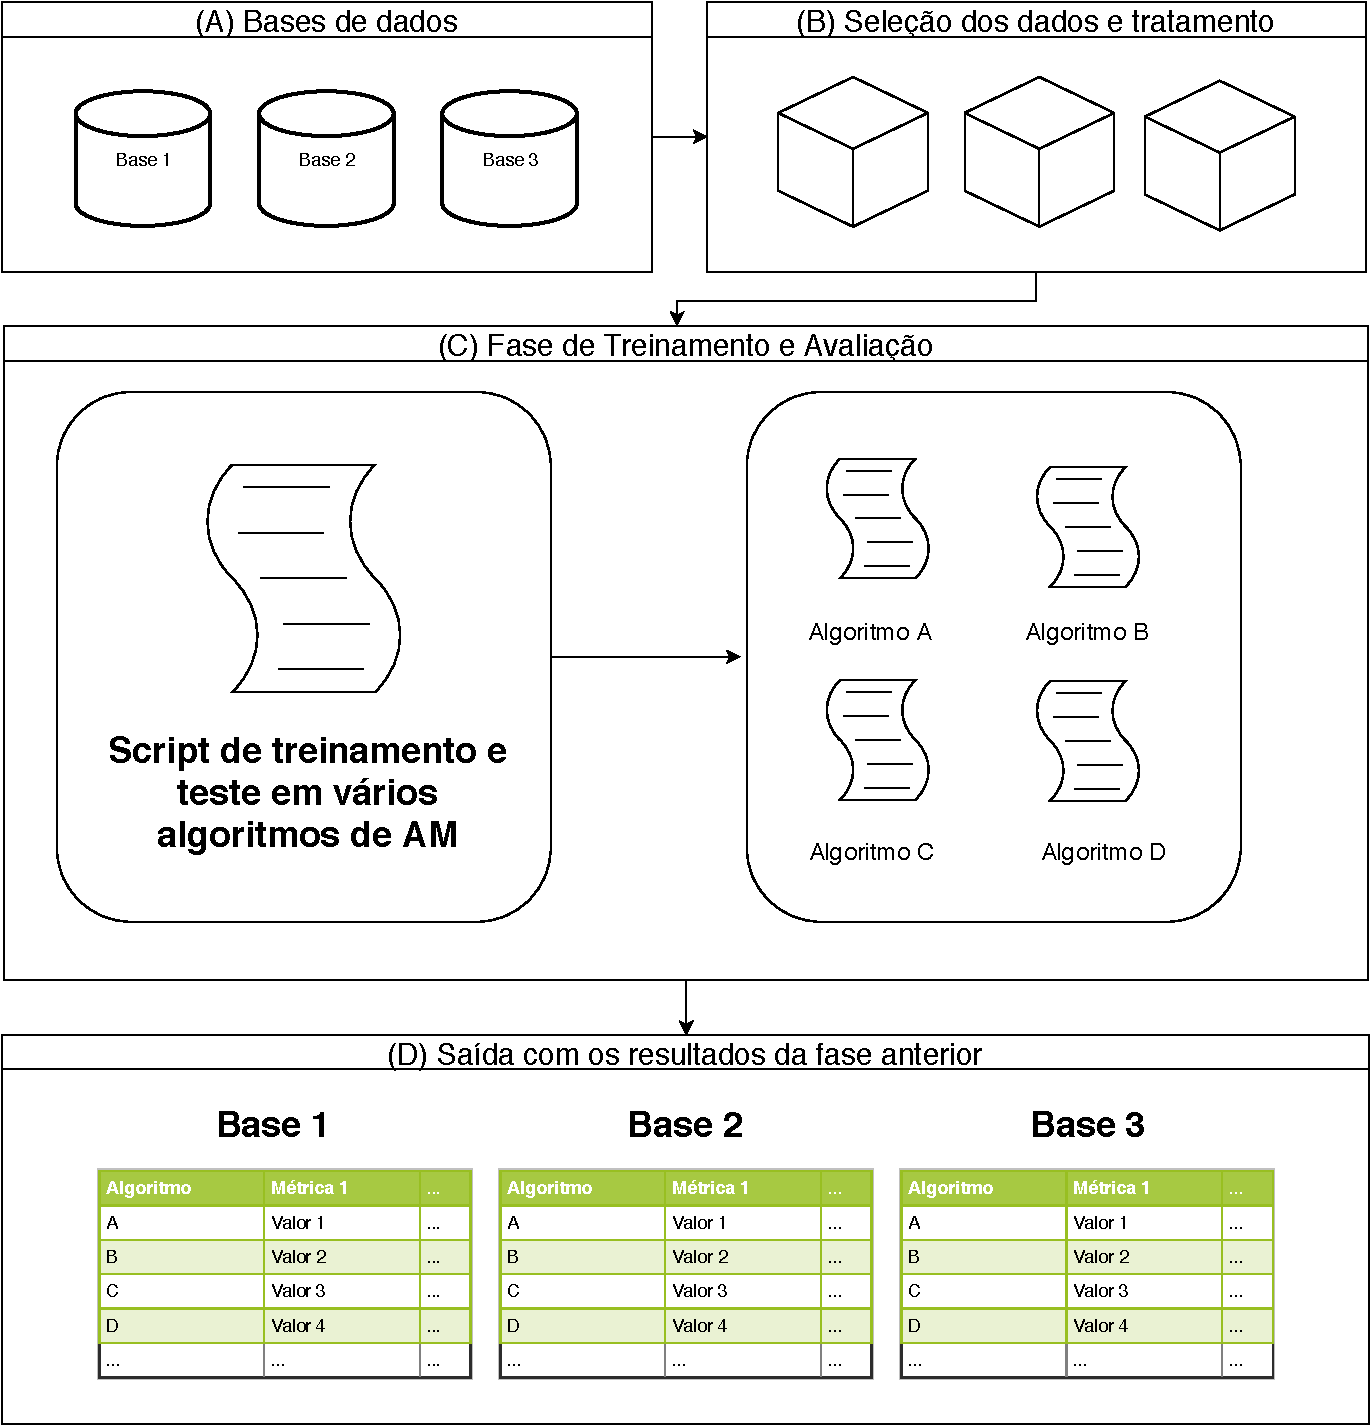
\includegraphics[width=1\textwidth]{desenvolvimento/Arquitetura.pdf}
    \caption{\label{fig:arquitetura}Arquitetura do projeto.}
    \legend{Fonte: Autor.}
\end{figure}

(isso aqui é só exemplo já que provavelmente devem haver mudanças na arquitetura)
Na Figura \ref{fig:arquitetura} as Bases de Dados (A), apresentadas na Seção \ref{basesdedados}, passam por uma fase de Seleção e Tratamento (B) para escolher, limpar e para a Fase de Treinamento e Avaliação (C)...

\section{Bases de Dados} \label{basesdedados}

Colocando links para acessar dps

HMC Software and Datasets (2008) https://dtai.cs.kuleuven.be/clus/hmcdatasets/ -- Funcat e Gene Ontology -- https://dtai.cs.kuleuven.be/clus/hmc-ens/

Catálogo Funcat -- https://web.archive.org/web/20081016031835/http://mips.gsf.de/projects/funcat/funcat20to21map -- https://www.researchgate.net/figure/Main-functional-categories-of-the-FunCat\_tbl1\_8230924

A Gene Ontology Tutorial in Python - https://www.nature.com/articles/s41598-018-28948-z -- https://pypi.org/project/goatools/

http://kt.ijs.si/DragiKocev/PhD/resources/lib/exe/fetch.php?media=clare2003.pdf

\section{Tecnologias Utilizadas}

\section{Algoritmos e Métricas de Avaliação}

\section{Configuração dos Experimentos}


\chapter{Resultados}

\section{Resultados na base abc}
\section{Resultados na base def}
\section{Resultados na base ghi}

\section{Análise e Discussão dos Resultados}

% ----------------------------------------------------------
% Finaliza a parte no bookmark do PDF
% para que se inicie o bookmark na raiz
% e adiciona espaço de parte no Sumário
% ----------------------------------------------------------
%\phantompart

% ---
% Conclusão (outro exemplo de capítulo sem numeração e presente no sumário)
% ---
\chapter[Conclusão]{Conclusão}
%\addcontentsline{toc}{chapter}{Conclusão}
% ---

\lipsum[31-33]

% ----------------------------------------------------------
% ELEMENTOS PÓS-TEXTUAIS
% ----------------------------------------------------------
\postextual
% ----------------------------------------------------------

% ----------------------------------------------------------
% Referências bibliográficas
% ----------------------------------------------------------
\bibliography{abntex2-modelo-references}

% ----------------------------------------------------------
% Glossário
% ----------------------------------------------------------
%
% Consulte o manual da classe abntex2 para orientações sobre o glossário.
%
%\glossary

% ----------------------------------------------------------
% Apêndices
% ----------------------------------------------------------

% ---
% Inicia os apêndices
% ---
%\begin{apendicesenv}

% Imprime uma página indicando o início dos apêndices
%\partapendices

% ----------------------------------------------------------
%\chapter{Quisque libero justo}
% ----------------------------------------------------------

%\lipsum[50]

% ----------------------------------------------------------
%\chapter{Nullam elementum urna vel imperdiet sodales elit ipsum pharetra ligula
%ac pretium ante justo a nulla curabitur tristique arcu eu metus}
% ----------------------------------------------------------
%\lipsum[55-57]

%\end{apendicesenv}
% ---

% ----------------------------------------------------------
% Anexos
% ----------------------------------------------------------

% ---
% Inicia os anexos
% ---
%\begin{anexosenv}

% Imprime uma página indicando o início dos anexos
%\partanexos

% ---
%\chapter{Morbi ultrices rutrum lorem.}
% ---
%\lipsum[30]

% ---
%\chapter{Cras non urna sed feugiat cum sociis natoque penatibus et magnis dis
%parturient montes nascetur ridiculus mus}
% ---

%\lipsum[31]

% ---
%\chapter{Fusce facilisis lacinia dui}
% ---

%\lipsum[32]

%\end{anexosenv}

%---------------------------------------------------------------------
% INDICE REMISSIVO
%---------------------------------------------------------------------
%\phantompart
\printindex
%---------------------------------------------------------------------

\end{document}
